\section{Basin-aware gain scheduling}\label{sec:basin-aware}

The schedule of Section~\ref{sec:feasibility} takes the largest gain whose steady command stays within the clip at every depth up to $\kappa\alim$; the residual authority that it leaves, and with it the disturbance that the cut tolerates, is whatever results. Sections~\ref{sec:bistability} and~\ref{sec:certificates} showed that this residual authority sets the basin. This section turns the tolerated disturbance into a design requirement.

\subsection{Formulation}\label{sec:ba-form}

At a spindle speed $n$, a gain $g$ and a depth $a$ are called admissible if
\begin{equation}\label{eq:admissible}
  a<\alim(n,g),\quad \bar b(n,a,g)\le(1-\rho)\Vmax,\quad \beta(n,a,g)\ge\beta_{\mathrm{req}},\quad a\le a_{\mathrm{phys}},
\end{equation}
that is, if the cut is linearly stable, its forced command keeps a voltage margin $\rho$, the certified kick $\beta$ of the averaged collocation model (C2, Section~\ref{sec:cert-c2}) is at least the required disturbance tolerance $\beta_{\mathrm{req}}$, and the depth is physically usable. The margin leaves room for runout, noise and errors of the model in the forced command (Section~\ref{sec:delayed-robust}); the certificate, however, is computed for the nominal forced command with the full clip, and it shrinks if these errors consume the margin. The basin-aware depth is
\begin{equation}\label{eq:arob}
  a_{\mathrm{rob}}(n;\beta_{\mathrm{req}})=\max_{g\in\mathcal G}\max\bigl\{a\in\mathcal A:\text{ all }a'\in\mathcal A\text{ with }a'\le a\text{ admissible with }g\bigr\},
\end{equation}
with $\mathcal A$ a grid of depths and $\mathcal G$ a grid of gains, and the gain that attains it is the basin-aware gain $g_{\mathrm{rob}}(n;\beta_{\mathrm{req}})$; where several gains attain it, the one with the larger smallest certified kick up to $a_{\mathrm{rob}}$, and then the smaller gain, is taken. As neither the forced command nor the certificate is monotone in the depth, every shallower depth of the grid is required, so that, as below a stability lobe, every grid depth up to $a_{\mathrm{rob}}$ can be used at that speed with one gain; the depths between grid points are linearly stable and keep the voltage margin, but are not certified. Equation~\eqref{eq:feas} chooses the gain for the largest linear limit under a constraint on the steady command; Eq.~\eqref{eq:arob} chooses it for the largest depth at which a disturbance of a given size is certified to be absorbed. Here $\rho=0.1$ and $a_{\mathrm{phys}}=2D=\SI{32}{\milli\metre}$.

The requirement $\beta_{\mathrm{req}}$ is an instantaneous velocity perturbation at any phase of the tooth period. As an equivalent displacement $\beta_{\mathrm{req}}/\omega_n$, 1, 2 and \SI{5}{\milli\metre\per\second} are 1.2, 2.5 and \SI{6.2}{\micro\metre}, and as an impulse $m\beta_{\mathrm{req}}$ at the four speeds of Section~\ref{sec:bistab-basin} they are 0.5--1.3, 1.0--2.5 and 2.4--\SI{6.3}{\percent} of the cutting impulse of one tooth period at \SI{16}{\milli\metre} [Eq.~\eqref{eq:impulse}]; near the linear limit the simulated basin of the DVF cut at $g=1500$ is 2.3--\SI{10.9}{\milli\metre\per\second} (Table~\ref{tab:basin}).
% src: beta / omega_n with omega_n = 2 pi x 129.3 rad/s: 1.231, 2.462, 6.154 um; impulse shares m beta / (F_y T) from Eq. (impulse) with src/params.py at 16 mm, 1090/1420/2500/2870 rpm: 0.48/0.62/1.09/1.25 %, 0.95/1.24/2.18/2.51 %, 2.38/3.10/5.46/6.27 % (recomputed); results/c1_basin.npz (worst-phase dv at 0.98 a_lim 2.34-10.88 mm/s)

\subsection{The basin-aware stability chart}\label{sec:ba-res}

Figure~\ref{fig:ba} shows the chart at 21 speeds from 500 to \SI{3000}{\rpm}, for gains of 0--\SI{3000}{\volt\second\per\metre} and depths on a \SI{2}{\milli\metre} grid, and Table~\ref{tab:ba} summarises it. The certificates were scanned with a reduced collocation order and every design point, every lower depth with a certified kick below $1.15\,\beta_{\mathrm{req}}$ and the failing depth were certified again with the default order; no design point had to be lowered (Supplementary Material).
% src: verification/paper/basin_aware.py/.json (protocol: GRID_RPM 500:125:3000, G_COARSE 0:250:3000 with refinement +-125, +-62.5, DEPTHS 2:2:32 mm, rho 0.1, a_phys 32 mm, BETA_REQ 1, 2, 5 mm/s; summary.*.corrected_down_speeds [] and upward_possible_speeds []; nred_vs_default: reduced/default 0.994-1.044)

Three features stand out. First, the linear limit at the chosen gain, not the voltage, binds at most speeds: the next grid depth is linearly unstable at 15, 17 and 15 of the 21 speeds for $\beta_{\mathrm{req}}=1$, 2 and \SI{5}{\milli\metre\per\second}, the physical depth binds at low speeds, where gains of 2500--\SI{3000}{\volt\second\per\metre} are usable, and the certificate binds at six speeds for \SI{5}{\milli\metre\per\second}. The voltage margin never binds directly, because the gain is chosen to respect it, but it is what stops a larger gain at two to four speeds. Second, the basin-aware gain departs from the authority gain in both directions (Fig.~\ref{fig:ba}b). Between 1500 and \SI{2500}{\rpm}, where the authority condition of Section~\ref{sec:feasibility} brings the steady command to the full \SI{9}{\volt}, it is lower: held to the same margin and certificate, the authority gain keeps them only up to \SI{4}{\milli\metre} there, as its forced command passes \SI{8.1}{\volt} near \SI{6}{\milli\metre}. At low speeds, and for 1 and \SI{2}{\milli\metre\per\second} also at high speeds, it is higher, because a larger gain raises the linear limit faster than it consumes the residual authority; for \SI{5}{\milli\metre\per\second} it is at or below the authority gain from \SI{1000}{\rpm} upwards. Third, the certified depths are comparable with the checked depths of Section~\ref{sec:feasibility}, which certify nothing: averaged over the 21 speeds, $a_{\mathrm{rob}}$ is 21.7, 19.9 and \SI{16.0}{\milli\metre} for the three requirements, against \SI{15.5}{\milli\metre} for $\achk$ (\SI{17.1}{\milli\metre} with gains up to \SI{3000}{\volt\second\per\metre}), and it falls below $\achk$ at 6, 7 and 11 speeds, mostly between 1500 and \SI{2500}{\rpm}. Unlike $\achk$, which stays $\kappa=0.9$ times below the linear limit, $a_{\mathrm{rob}}$ has no explicit depth margin: its median ratio to $\alim(g_{\mathrm{rob}})$ is 0.97, 0.97 and 0.91 for the three requirements, the last close to $\kappa$.
% src: verification/paper/basin_aware.json (summary.1/2/5: primary_binding_counts_grid21 {linear 15, a_phys 6}, {linear 17, a_phys 3, certificate 1}, {linear 15, certificate 6}; gain_limited_by_primary_grid21 voltage margin 4/3/2; g_star_by_rpm; per_speed.*.auth_under_basin_criteria a_rob 4 mm at 1500-2500 rpm; per_speed.2500.designs.1.next_higher_evaluated_gain fail_bbar_V 8.57 at 6 mm; a_rob_mm_grid21 mean 21.71/19.90/16.00; a_chk_mm_grid21_mean 15.50; auth_g3000 a_chk mean 17.13 (recomputed over the 21 speeds); a_rob_below_a_chk_speeds 6/7/11; per_speed.*.designs.*.a_rob_over_a_lim_at_g median 0.973/0.970/0.909 over the 21 speeds, recomputed; designs.*.voltage_margin_violated_between_grid_depths false at all 63 designs; g_star_by_rpm against auth_g1500.g: 5 mm/s g_rob <= g_auth from 1000 rpm)

\begin{table}[!tbp]
  \centering
  \caption{Basin-aware stability chart over 21 speeds (500--\SI{3000}{\rpm}; gains 0--\SI{3000}{\volt\second\per\metre}; voltage margin $\rho=0.1$; depth grid \SI{2}{\milli\metre}; $a_{\mathrm{phys}}=\SI{32}{\milli\metre}$). Binding: the condition that fails at the next grid depth (linear limit / $a_{\mathrm{phys}}$ / certificate). Validation: the smallest ratio to $\beta_{\mathrm{req}}$ of the simulated critical kick, smallest over four phases, at six speeds.}
  \label{tab:ba}
  \small
  \begin{tabular}{@{}lcccc@{}}
    \toprule
    $\beta_{\mathrm{req}}$ & $a_{\mathrm{rob}}$ (\si{\milli\metre}) & Binding & $a_{\mathrm{rob}}/\achk$ & Validation\\
    (\si{\milli\metre\per\second}) & mean (range) & & median & \\
    \midrule
    1 & 21.7 (10--32) & 15 / 6 / 0 & 1.26 & 2.75\\
    2 & 19.9 (10--32) & 17 / 3 / 1 & 1.23 & 2.78\\
    5 & 16.0 (10--26) & 15 / 0 / 6 & 1.00 & 2.27\\
    \midrule
    $\achk$, Section~\ref{sec:feasibility} & 15.5 (12.6--24.1) & -- & 1 & --\\
    \bottomrule
  \end{tabular}
\end{table}
% src: verification/paper/basin_aware.json (summary.*: a_rob_mm_grid21, primary_binding_counts_grid21, a_rob_over_a_chk_grid21.median 1.258/1.230/1.000; validation_summary.*.worst_crit_kick_over_beta_req_min 2.750/2.780/2.272; per_speed.*.auth_g1500.a_chk_mm 12.57-24.07)

\begin{figure}[!tbp]
  \centering
  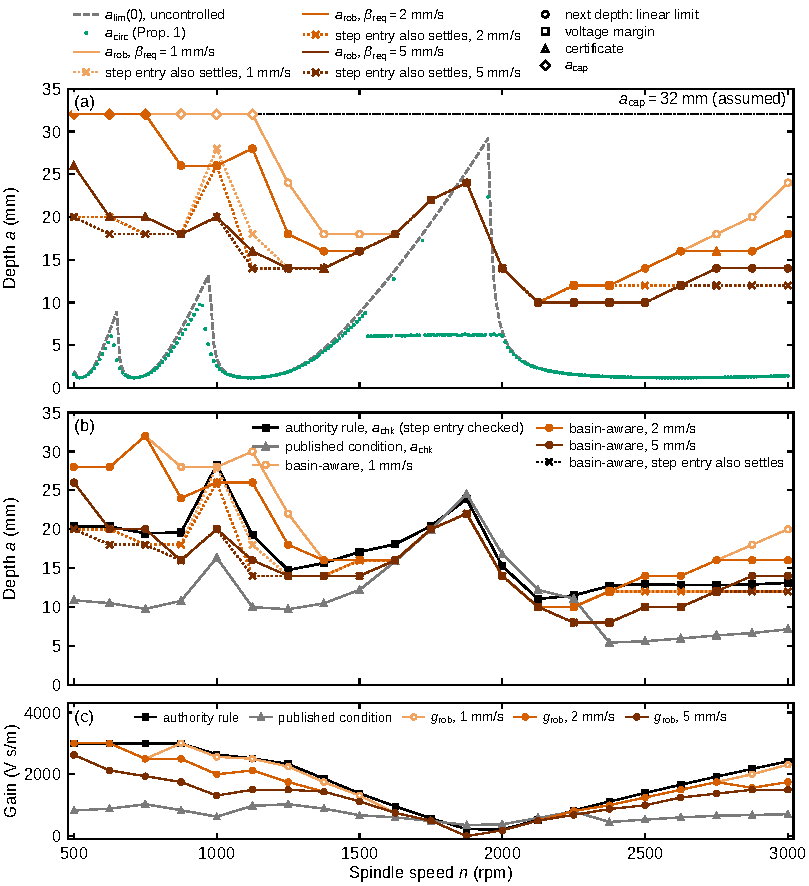
\includegraphics[width=0.86\textwidth]{figures/fig_basin_aware.pdf}
  \caption{Basin-aware stability chart. (a)~Largest depth $a_{\mathrm{rob}}$ up to which every grid depth is linearly stable, keeps \SI{10}{\percent} of the voltage free and has a certified kick of at least $\beta_{\mathrm{req}}=1$, 2 or \SI{5}{\milli\metre\per\second} (C2, averaged collocation model), with the condition that fails at the next grid depth (markers); for comparison, the authority schedule of Section~\ref{sec:feasibility} ($g\le\SI{1500}{\volt\second\per\metre}$: linear limit and checked depth), the depth of the published condition, Eq.~\eqref{eq:pub}, the uncontrolled limit and the depth $a_{\mathrm{circ}}$ below which the averaged delay model attracts every solution at the authority gains (Proposition~\ref{prop:circle}). (b)~Basin-aware gains and the authority-schedule gain.}
  \label{fig:ba}
\end{figure}

\subsection{Validation in the simulator}\label{sec:ba-valid}

At six speeds (750, 1125, 1375, 2000, 2500 and \SI{2875}{\rpm}) the design points were simulated with the \SI{9}{\volt} clip and the full surface memory. The simulated critical kick, smallest over four phases a quarter of a tooth period apart, exceeds $\beta_{\mathrm{req}}$ by factors of at least 2.75, 2.78 and 2.27 for 1, 2 and \SI{5}{\milli\metre\per\second}, or 1.6--6.9 times the certified kick, and kicks of exactly $\beta_{\mathrm{req}}$ at all 16 phases never caused chatter (0 of 96 for each requirement). The face entry settles at every design point of the chart. The step entry from rest, however, ends in chatter at 14, 12 and 7 of the 21 design points: the chart certifies the settled cut against disturbances, not the entry, which has to be gentle (Section~\ref{sec:bistab-map}) or certified separately along $-\xi_p(0)$ (Section~\ref{sec:cert-c2}), which succeeds only at shallow depths.
% src: verification/paper/basin_aware.json (validation_summary.1/2/5: points 6, all_above_beta_req true, worst_crit_kick_over_beta_req_min 2.750/2.780/2.272, td_over_cert 1.63-6.95, kicks_of_beta_req_chattering 0 of 96; summary.*.face_entry_chatters_at_design_rpm [], step_entry_chatters_at_design_rpm 14/12/7 speeds)
